\chapter{Domain Decomposition}
\label{chap:domain-decomp}

\newcommand{\lave}{\langle \lambda \rangle}
\newcommand{\lmave}{\langle \overline{\lambda} \rangle}
\newcommand{\lroot}{\| \lambda \|}
\newcommand{\deltap}{\delta{p_{i,j}}}
\newcommand{\dpmax}{\delta{p_i^{max}}}
\newcommand{\pmax}{{p_i^{max}}}
\newcommand{\lmax}{{\lambda_i^{max}}}
\newcommand{\pbar}{\overline{P}}
\newcommand{\xx}{\frac{\beta ||\lambda^{max}|| + \mu}{\beta
    ||\overline{\lambda}|| + \mu} }
\newcommand{\yy}{ \frac{\sum_{i=0}^M ||{\lambda^{max}}||^i}{\sum_{i=0}^M
    ||\overline{\lambda}||^i} }

\section{Background}
Particle based Monte Carlo (MC) methods for neutron transport are becoming an
increasingly active area of research in the reactor physics
community. Traditional reactor core analysis codes are based on various
discretizations of the deterministic transport equation, viz. so-called PN, SN,
and Method of Characteristics (MOC) formulations. Monte Carlo methods, however,
offer several potential advantages to these traditional formulations,
particularly in areas that tend to encumber the practical adoption of transport
tools to new classes of problems --- viz. the avoidance of complex meshing for
complicated geometries, the simplification of the cumbersome multi-group cross
section generation process, and, perhaps most importantly, the potentially
easier adaptability to the extreme levels of concurrency that are likely to
characterize beyond-petascale HPC architectures \cite{jkns-chang-2009}. Reactor
MC simulations, though, are notoriously expensive computationally
\cite{mc-hoogenboom-2009, pnst-wagner-2011, physor-kelly-2010}, and a number of
algorithmic and implementation challenges remain before they can be robustly
applied to practical reactor analysis.

One of these challenges involves developing parallel methods with dramatically
reduced per-node memory footprints (e.g. \cite{pnst-romano-2011}). Existing
production MC codes for reactor analysis are either implemented serially or
carry out parallelization by simple replication --- i.e. distributing batches of
particles to processors while replicating and synchronizing the key data
structures across nodes. This approach is relatively easy to implement and has
excellent scalability properties. However, for robust reactor calculations, the
required memory footprint in general far exceeds node-level memory
resources. Thus, even the largest reactor MC calculations to date have been
forced to employ a number of simplifications and approximations in order to fit
standard reactor physics calculation in memory \cite{physor-kelly-2010}.

In reactor applications the majority of memory is consumed by two types of data
--- 1) interaction cross section libraries and 2) interaction tallies for
pre-defined geometric regions \cite{mc-hoogenboom-2009}. The cross section data
libraries are read into main memory and accessed randomly during the tracking of
an individual neutron. This data needs to be accessible to each process and can
be more or less significant depending on the specific application. Standard
Light Water Reactor (LWR) analyses, for example, require data for several
reaction types for each of 200--400 isotopes at approximately 50 temperature
intervals and 200,000 energy points. At eight bytes per data point this memory
can exceed 100GB. Existing research into compact functional representations has
the potential to reduce this footprint significantly, but this is currently a
topic of research and developing algorithmically creative ways of handling cross
section data remains an important technique for reducing the total memory cost
\cite{pnst-brown-2011}.

For LWR applications in particular, the tallies are an even more significant
consumer of memory. We conservatively estimate that a robust LWR analysis would
require approximately a factor of fifty greater than the 8GB reported in the
landmark calculations of Kelly et al. \cite{physor-kelly-2010} --- specifically,
an additional 5 axial levels and and a factor of 10 in radial rings per fuel pin
(to treat radial temperature profiles and self-shielded absorbers) --- for a
total of 500GB of memory. Unlike the cross section libraries, tally data is
write only and requires a relatively small amount of data to be transferred for
each update.

In this paper we focus on algorithmic issues related to the reduction of the
local tally memory. Two classes of strategies have been proposed to address this
problem --- what we loosely refer to as \emph{data decomposition} and
\emph{domain decomposition}. Data decomposition could take many forms, but the
basic approach would involve the same naturally parallel by-particle
parallelization strategy as is currently employed together with a set of
dedicated \emph{tally servers} that continuously receive tally updates from the
tracking processors (e.g. with one-side operations or by running a continuous
receive loop).  The spatial decomposition of the tallies is in general arbitrary
and the data sent from the tracking processors could be carried out with
non-blocking MPI send operations to maximize overlap in
communication/computation. Of course, this idea could be extended to
non-disjoint processor sets, but for illustrative purposes it is perhaps easiest
to imagine them as distinct.

Domain decomposition on the other hand associates a contiguous region of
physical space with each processing element (or node). Each processor then owns
the subset of tallies for the corresponding region of physical space. This
approach is potentially made efficient with a more complex parallelization
strategy where each processor only tracks the particles that are passing through
its own portion of the domain.  However, new complexities emerge --- fast
neutrons travel long distances before absorption, and thus the local leakage
rates (probability of a neutron leaving a partition before being absorbed) are
relatively large. This requires intermediate data exchange \emph{stages} where
particles are moved to adjacent processors, potentially leading to significant
communication costs and non-trivial load imbalances.

In a recent work by Siegel et al. \cite{jcp-siegel-2012-1}, the authors attempt
to quantify this cost, exploring the feasibility of carrying out efficient
domain decomposition in a parameter regime relevant to Light Water Reactor (LWR)
analysis.  Key scaling regimes are identified and performance estimates are
carried out over a range of characteristic parameters. The results demonstrate
that for the model problem good performance is expected for reasonable effective
latency and bandwidth values for partition particle densities as low as $10^4$
per node (e.g. on the BG/P platform).  This analysis takes an important step
toward quantifying the key theoretical issues and establishing the feasibility
of carrying out robust LWR calculations with MC methods.


However, the analysis in \cite{jcp-siegel-2012-1} does not address the impact of
initial particle imbalances and small variations in local leakage rates on
evolving particle distributions.  If particle communication costs are
potentially manageable in light of typical machine bandwidth and latencies, to
what extent will load imbalances negatively impact performance to the point
where such an approach is no longer a practical alternative?  Establishing a
quantitative foundation for this performance penalty will greatly facilitate
weighing tradeoffs in deciding the best path forward among various approaches
for next-generation MC codes.  In this paper we address this issue directly by
attempting to quantify the effect of particle load imbalances and typical
material inhomogeneities on the performance of domain decomposed MC algorithms.


\section{Analysis}
\subsection{Problem definition}
\label{sec:definition}

To fully define the problem, begin with a domain $X$ segmented into $N$
non-overlapping partitions $X = \cup x_j, j=1...N$. If we denote the initial
number of particles on partition $x_j$ as $p_{0,j}$, then the initial global
particle count $P_0$ is given by:
\begin{equation}
  \label{eq:globalP}
  P_0 = \sum_{j=1}^{N} p_{0,j}.
\end{equation}
For simplicity, assume that each partition is mapped to a single processing
element on a three-dimensional virtual Cartesian topology of $N$ processors. In
this work we thus use the terms \emph{processor}, \emph{partition}, and
\emph{process} interchangeably.

On a given partition, particles owned by that partition are advanced through a
sequence of interactions until they are either 1) absorbed or 2) reach a
processor boundary. For optimal performance particles that reach the boundary
are buffered locally until all particle trajectories are computed, and are
subsequently exchanged with neighbor processors. We refer to the particle
exchange phase of this process as a \emph{stage}, and to a complete set of
stages (i.e. until all particles are absorbed) as a \emph{cycle}. At the end of
each cycle, the fission source is updated and the next cycle begins.

Define the particle {\it local leakage $\lambda$} on each $x_j$ for a given
stage $i$ as
\begin{equation*}
  \lambda_{i,j} = \frac{\mbox{ number of particles leaving $x_j$ at stage
      $i$}}{\mbox{ number of particles starting in $x_j$ at stage $i$}}.
\end{equation*}
The goal of this analysis is to estimate the impact of initial particle load
imbalances and spatially varying local leakage values on previous performance
estimates of domain-decomposed LWR simulations.  We refer to the perfectly load
balanced, constant leakage scenario as the \emph{ideal} case. This was explored
in depth in \cite{jcp-siegel-2012-1}, where it was shown that communication
costs imposed a reasonable penalty on overall simulation time for a broad range
of relevant parameter values.

An important followup question, though, is to what extent load imbalances will
affect overall performance. In \cite{jcp-siegel-2012-1} the analysis was carried
out in the ideal case, and it was assumed that load imbalances could be handled
efficiently by standard re-partitioning algorithms. Here we aim to quantify the
cost of load balance, both to further gauge the feasibility of domain-decomposed
MC codes, as well as to provide a decision-making metric for carrying out load
balancing in production codes.

Following \cite{scott-2005} we first define the \emph{load balance} $\Gamma_i$
at each stage $i$ as
\begin{equation}
  \Gamma_i = \frac {\overline{P}_i}{p_i^{max}},
\end{equation}
where \[ \overline{P}_i = \frac{1}{N}\sum_{j=1}^{N} p_{i,j} \] and $p_i^{max}$
denotes the maximum particle count at stage $i$.  The amount the load balance
$\Gamma_i$ differs from the ideal case $\Gamma = 1$ measures the relative
difference between the highest particle and average particle counts:
\begin{equation}
  1- \Gamma_i = \frac{p_i^{max} - \overline{P}_i}{p_i^{max}}
\end{equation}
Note that unlike \cite{scott-2005} we express the load imbalance in terms of
particle densities rather than execution time. Their equivalence will be argued
in the following section.

We seek to estimate a related but distinct quantity --- an upper bound for the
difference between the total per-cycle simulation time of the non-ideal case and
the ideal case. We define this normalized difference as the {\it load imbalance
  penalty} $\Delta$:
\begin{equation}
  \Delta = \frac{\tau' - \tau}{\tau} = \frac{\tau'}{\tau} - 1,
\end{equation}
where $\tau$ denotes the total per-cycle simulation time in the ideal case, and
$\tau'$ for the non-ideal case.  Note that an expression for $\Delta$ must
include both the particle tracking as well as the communication costs across all
stages of a given cycle. While related to the per-stage particle load balance,
the load imbalance penalty is a distinct quantity.

\subsection{Basic properties}

Given this simple problem definition above, it is clear that, for purely
reflective boundary conditions (a good approximation for reflectors in power
reactors) the \emph{global} number of particles at any \emph{stage} is given by
\begin{equation}
  \label{eq:pg}
  P_{i+1} = \sum_{j=1}^N p_{i+1,j} = \sum_{j=1}^N \lambda_{i,j}
  p_{i,j} \hspace{.5in} i=0,1,\dots M,
\end{equation}
where $M$ denotes the final stage in the cycle --- i.e. when all particles are
absorbed and none remain. We emphasize again that $P_i$ denotes the global
particle count at stage $i$ while $p_{i,j}$ denotes the local particle count on
partition $j$ at stage $i$.

To estimate $\tau'$, the per cycle simulation time in the non-ideal case, we
seek an expression for the \emph{local} particle distribution --- i.e. the
number of particles on each partition $x_{j}$ at stage $i$. Assuming isotropic
leakage, the neutron count on a partition is given by:
\begin{equation}
  \label{eq:pl}
  p_{i+1,j} = \frac{1}{6} \left( \lambda_{i,j1}p_{i,j1} + \lambda_{i,j2}p_{i,j2}
  + \cdots + \lambda_{i,j6}p_{i,j6} \right)
\end{equation}
\noindent where $j1,j2 \cdots j6$ denote the six immediate neighbors of
partition $j$ on a Cartesian lattice. Equation \eqref{eq:pl} simply states that, in
advancing stages, a given partition receives $1/6th$ of the leaked particles
from each of its six neighbors on a Cartesian grid.

Equation \eqref{eq:pl} shows that the evolution of the local particle
distributions depends on the detailed alignment of the local particle counts and
the local leakage rates. To reduce it further requires additional
assumptions. We start by noting that, in an LWR, the neutron spectrum and
material heterogeneities are roughly constant from partition to partition (this
property is demonstrated using simulation data in Section 3). This observation
makes the case of approximately spatially uniform local leakages of great
practical interest in the present context, and thus we initially consider the
case of $\lambda_{i,j} = \lambda_i$. Note that we still expect non-trivial
per-stage variation in leakages as neutron energies will shift toward the
thermal range with increasing stages. Important model corrections for small
spatial variations in $\lambda$ will be considered in \autoref{sec:var_leak}.


For spatially constant $\lambda$, \eqref{eq:pg} then becomes
\begin{align}
  \label{eq:pg2}
  P_{i} &= \sum_{j=1}^N \lambda_{i-1} p_{i-1,j} = \lambda_{i-1}
  \sum_{j=1}^Np_{i-1,j} = \lambda_{i-1} P_{i-1} \\
  &= \lambda_{i-1} \lambda_{i-2} \dots \lambda_{0} P_0 \\
  &\sim {\lave}^{i} P_0 \hspace{2in} i=1,2,\dots M
\end{align}
where $\lave$ is defined as the geometric mean of the leakage rate,
\begin{equation}
  \label{eq:cycle_mean}
  \lave = \sqrt[M]{\lambda_{M-1}\lambda_{M-2} \dots \lambda_{0} }.
\end{equation}
Equation \eqref{eq:pl} then simplifies to

\begin{equation}
  \label{eq:meanp}
  p_{i+i,j} = \frac{\lambda_i}{6} \left( p_{i,j1} + p_{i,j2} + \cdots + p_{i,j6}
  \right)
\end{equation}
Equation \eqref{eq:meanp} shows that, for spatially constant $\lambda$, at each
subsequent stage each partition has the average value of the total leaked
particles from the neighboring partitions in the previous stage.  Equation
\eqref{eq:pg2} shows that, in the case of constant $\lambda$, the particle load
imbalance does not affect the number of stages required to complete a cycle,
which can be estimated by setting $P_i = 1$ in \eqref{eq:pg2}:
\begin{equation}
  \label{eq:kfinal}
        {\lave}^M P_0 = 1 \implies M \sim -\frac{\log P_0}{\log \lave}.
\end{equation}
Both properties are used in the analysis that follows.

\subsection{Expression for $\tau$}

Given these basic properties, we first seek an estimate of the total per-cycle
cost in the idealized case of an initial even distribution of particles and
spatially constant $\lambda$.  This is accomplished by decomposing $\tau$ into a
local work $\tau_l$ and inter-processor communication $\tau_c$ component as
\begin{equation}
  \tau = \tau_l + \tau_c.
\end{equation}
In the case of perfect load balancing and assuming a roughly equal distribution
of track length and neutron spectra across partitions (i.e. our earlier
assumption of constant $\lambda$), the local work $\tau_l$ should be roughly
proportional to the total number of particles tracked on a partition in a given
cycle,
\begin{equation}
  \label{eq:loc_work}
  \tau_{l} = \mu \sum_{i=0}^{M} \overline{P}_{i},
\end{equation}
where the constant $\mu$ is a measure of the tracking time per particle, and
where it is understood that the particle count $p_{i,j}$ is the same on any
given partition, since all partitions are equivalent in the ideal case.

The communication time $\tau_c$ can be further decomposed into a latency and
bandwidth component \cite{jcp-siegel-2012-1}.  For each cycle, a total of $M$
messages need to be sent to each processor's six neighbors, so in general the
total time per cycle due to message latency can be modeled as $\sim 6 \alpha M$,
where $\alpha$ is some measure of the effective application-level latency for a
single send.

If we ignore the dependence of $\lambda$ on stage, by definition $\lambda
\overline{P}_i$ particles are sent from each processor at stage $i$, the total
number of particles sent in a cycle from any processor is $\lambda \sum_i
\overline{P}_i$. Thus, the bandwidth term can be roughly modeled as $\beta
\lambda \sum_i \overline{P}_i$, where $\beta$ denotes the effective inverse
bandwidth for nearest-neighbor exchanges (expressed in $\frac{time}{particle}$).

When we account for stage dependence $\lambda$ is replaced by $||\lambda||$,
defined as the solution to the $M$-th order polynomial:
\begin{equation}
  \label{eq:lmean}
  \sum_{i=1}^M ||\lambda||^i = \lambda_0 + \lambda_1\lambda_0 + \cdots +
  \lambda_M\lambda_{M-1}...\lambda_0.
\end{equation}
The latency term can then be written as:
\begin{align*}
  \beta \sum_{i=0}^M \lambda_i \overline{P}_i &= \beta(\lambda_0 \overline{P}_0
  + \lambda_1 \overline{P}_1 + \dots \lambda_M\overline{P}_M)  \\
  &= \beta(\lambda_0 \pbar_0 + \lambda_1 \lambda_0 \pbar_0 + \dots +
  \lambda_M\lambda_{M-1}...\lambda_0 \pbar_0) \\
  &=\beta\pbar_0(\lambda_0 + \lambda_1\lambda_0 + \dots) \\
  &= \beta\pbar_0\sum_{i=1}^M ||\lambda||^i  \\
  &\sim \beta\pbar_0\frac{||\lambda||}{1-||\lambda||}
\end{align*}

Using these relations together with \eqref{eq:kfinal} then yields the following
expression for the total communication time:
\begin{equation}
  \label{eq:tot_comm}
  \tau_c = -6 \alpha \frac{\log P_0}{\log \lave} +
  \beta\pbar_0\frac{||\lambda||}{1-||\lambda||}
\end{equation}
where it is understood that the last term in the summation is zero --- i.e. no
particles are sent after the final stage --- and that it is included as a
notational convenience.  Using the same approach on \eqref{eq:loc_work} and
combining with \eqref{eq:tot_comm} gives the final expression for total
simulation time in the idealized case:
\begin{equation}
  \label{eq:tau1}
  \tau = -6 \alpha \frac{\log P_0}{\log \lave} + (\mu + \beta
  \lroot)\frac{\overline{P}_0}{1-\lroot},
\end{equation}

\subsection{Expression for $\tau'$}

We now seek an estimate for the total cycle time $\tau'$ in the presence of an
initial load imbalance.  For convenience we first express $p_{i,j}$ as a
combination of partition mean and fluctuating parts. That is,
\begin{equation}
  \label{eq:mean}
  \deltap = p_{i,j} - \overline{P}_i
\end{equation}
When a load imbalance is present the partition with the largest particle count
controls the total performance cost.  If we denote the particle count on this
process as $p^{max}_i = \overline{P}_i + \dpmax$, then by analogy with
\eqref{eq:tau1} it is clear that the load-imbalanced performance cost is:
\begin{align}
  \label{eq:eta}
  \tau' &= -6 \alpha \frac{\log P_0}{\log \lave} + (\mu + \beta \lroot)
  \sum_{i=0}^{M} (\overline{P}_i + \dpmax) \\
  &= \tau + (\mu + \beta \lroot) \sum_{i=0}^{M}\dpmax
\end{align}
where the equivalence of the latency terms, i.e. \eqref{eq:kfinal}, has been
used.

While we cannot directly evaluate the sum of $\delta p_i^{max}$, a simple upper
bound can be derived by recognizing that, assuming roughly equal leakage to each
neighbor, the largest possible value of $p$ at stage $i+1$ occurs if all six
neighbors of a partition contain $\dpmax$ particles. Thus,
\begin{equation}
  \label{eq:ub}
  \delta p^{max}_{i+1} \le \lambda_i \delta p^{max}_i.
\end{equation}
Substituting the right hand side of \eqref{eq:ub} for each element of the sum
\eqref{eq:delta1} yields:
\begin{align*}
  \sum_{i=0}^M \delta p_i^{max} &\le \delta p_0^{max} + \lambda_0\delta
  p_0^{max} + \dots + \lambda_M\delta p_0^M  \\
  &= \delta p_0^{max}(1 + \lambda_0 + \lambda_0\lambda_1 + \dots) \\
  &\sim \frac{\delta p_0^{max}}{1-||\lambda||}
\end{align*}
Equation \eqref{eq:eta} then becomes
\begin{equation}
  \label{eq:tauprime}
  \tau' = \tau + (\mu + \beta \lroot) \frac{\delta p_0^{max}}{1 - ||\lambda||}.
\end{equation}

\subsection{Expression for $\Delta$}

Using \eqref{eq:eta} and \eqref{eq:tauprime} we get the following expression for
$\Delta$:
\begin{equation}
  \label{eq:delta1}
  \Delta = \frac{\tau'-\tau}{\tau} \le \frac{\delta p_0^{max}} { (1-\lroot)
    \epsilon + \overline{P_0} }
\end{equation}
where $\epsilon$ measures the relative importance of latency relative to
bandwidth and tracking timescales, i.e.
\begin{equation}
  \label{eq:latency}
  \epsilon = \frac{6 \alpha}{\mu + \beta \lroot} \frac{\log P_0}{\log \lave}
\end{equation}
which is presumed to be small for typical problem sizes and parameter regimes
(e.g. see \cite{jcp-siegel-2012-1}) but which is retained here for the sake of
generality.  Note that \eqref{eq:delta1} implies that
\begin{equation}
  \label{eq:delta3}
  \Delta \le \frac{\delta p_0^{max}}{\overline{P_0}} =\frac{1} {\Gamma_0} - 1,
\end{equation}
which should be a good approximation for applications where the latency term is
much smaller than the bandwidth and tracking terms.

Assuming spatially constant $\lambda$, then, and given isotropic neutron local
leakage and constant mean tracking rates per partition, we can establish an
upper bound for $\Delta$ entirely in terms of the initial particle
configuration.

\section{Variable leakage rates}
\label{sec:var_leak}

Equation \eqref{eq:delta1} should give a reasonable estimate for reactor applications
across a range of parameter values, where material inhomogeneities are roughly
equally distributed and thus local leakage rates show very little
variation. However, it fails to capture a critical effect that emerges as we
move to smaller partition sizes, and which sets an important limit on the
utility of the domain-decomposed approach.  To see this we explicitly account
for spatially variant, non-constant leakage in the formulation of the model.

Consider a distribution of leakage rates across partitions at a given stage with
a maximum value defined as:
\begin{equation}
  \lambda^{max}_i = \max \left\{\lambda_{i,j} : 1 \le j \le N\right\}
\end{equation}
In estimating the computation time for this scenario compared to the ideal case
(i.e. calculating $\Delta$), the question arises of what corresponding spatially
constant value of $\lambda$ should be used for the ideal case. Several options
are reasonable, but here we choose a mean value that preserves
stages. Specifically, if we define a particle-weighted mean leakage as:
\begin{equation}
\label{eq:pmean}
\overline{\lambda}_i := \frac{\sum_{j=1}^{N} p_{i,j} \lambda_{i,j}}{P_i}
\end{equation}
then the ideal and non-ideal cases are guaranteed to have the same number of
global particles at successive stages: \[ \frac{P_{i+1}}{P_i} =
\frac{1}{P_i}\sum_{j=1}^N \lambda_{i,j} p_{i,j} = \overline{\lambda}_i \].
Following \eqref{eq:ub}, then, the largest possible particle count at stage $i$
occurs on partition $x_j$ if on its six neighbors $\pmax$ coincides with
$\lmax$.  That is,
\begin{equation}
  \label{eq:ub2}
  p^{max}_{i+1} \le \lmax \pmax.
\end{equation}
This relation then allows us to derive an upper bound for $\tau'$ in the case of
variable $\lambda$:
\begin{align*}
  \tau' &\le 6\alpha\frac{\log P_0}{\log \lmave} + \beta \sum_{i=0}^{M} \lmax
  \pmax + \mu \sum_{i=1}^M \pmax  \\
  &= 6\alpha\frac{\log P_0}{\log \lmave} + (\mu + \beta ||\lambda^{max}||)
  \sum_{i=0}^{M} \pmax
\end{align*}
where $||\lambda^{max}||$ is defined analogous to \eqref{eq:lmean}:
\begin{equation*}
  \sum_{i=1}^M ||\lambda^{max}||^i = \lambda^{max}_0 +
  \lambda^{max}_1\lambda^{max}_0 + \cdots +
  \lambda^{max}_M\lambda^{max}_{M-1}...\lambda^{max}_0.
\end{equation*}
This then yields the following upper bound for the load imbalance:
\begin{equation}
  \label{eq:delta4}
  \Delta \le \frac{ (\mu + \beta ||\lambda^{max}||)\sum_{i=0}^M \delta
    p_i^{max}} {6\alpha\frac{\log P_0}{\log \left<\overline{\lambda}\right>} +
    (\mu + \beta
    ||\overline{\lambda}||)\frac{\overline{P_0}}{1-||\overline{\lambda}||}}
\end{equation}
Note that the term $\sum_{i=0}^M \delta p_i^{max}$ can be written in terms of
$p_0^{max}$ as:
\begin{align*}
  \sum_{i=0}^M \delta p_i^{max} &= \delta p_0^{max} + \lambda_0^{max} \delta
  p_0^{max} + \lambda_0^{max} \lambda_1^{max}\delta p_0^{max} + \dots \\
  &= \delta p_0^{max}(1 + \lambda_0^{max} | \lambda_0^{max}\lambda_1^{max} +
  \dots \\
  &= \delta p_0^{max}\sum_{i=1}^M ||\lambda^{max}||^i
\end{align*}

If for convenience we replace $\sum_{i=1}^M ||\lambda^{max}||^i$ by its
continuous representation $\frac{1}{1-||\lambda||}$ , then \eqref{eq:delta4}
implies that:
\begin{equation}
  \label{eq:delta5}
  \Delta \le C \frac{p_0^{max}}{\overline{P}_0} = \frac{C}{\Gamma_0} - 1.
\end{equation}
where the quantity C, defined as,
\begin{equation*}
  C = \frac{(\beta ||\lambda^{max}|| + \mu)}{(\beta ||\overline{\lambda}|| +
    \mu)} \frac{(1 - ||\overline{\lambda}||)}{(1-||\lambda^{max}||)},
\end{equation*}
can be seen as a "correction factor" relative to \eqref{eq:delta3} --- clearly,
when $||\overline{\lambda}|| = ||\lambda^{max}||$, \eqref{eq:delta4} reduces to
\eqref{eq:delta3}.

Note however that the Taylor Series expansion used in the derivation of
\eqref{eq:delta5},
\begin{equation*}
  \frac{1}{1-x} = 1 + x + x^2 + \dots + x^M,
\end{equation*}
even for large M is a poor approximation for $x$ extremely close to 1. While
this will not be a problem for average values of $\lambda$ in reactor
applications, we must allow for the possibility that $\sum_{i=0}^M
||\lambda^{max}||^i$ approaches its true upper bound of $M$ (i.e. the
\emph{maximum} leakage in each stage is 1). Thus, a potentially more accurate
version of C is:
\begin{equation*}
  C = \frac{(\beta ||\lambda^{max}|| + \mu)}{(\beta ||\overline{\lambda}|| +
    \mu)} \frac{\sum_{i=0}^M ||{\lambda^{max}}||^i}{\sum_{i=0}^M
    ||\overline{\lambda}||^i}
\end{equation*}

The greater the spatial variation in leakage rates the more the system bandwidth
and neutron tracking rates factor into the performance. The implications of
these formulas are explained in the simple tests below, where we aim to estimate
C as a function of the main problem parameters.

\section{Evaluation of model}

For a given initial particle configuration, evaluation of the model equation
\eqref{eq:delta4} requires estimates for particle tracking rate $\mu$,
application-level inverse bandwidth $\beta$ and latency $\alpha$, and local
leakage rate estimates from which to compute $||\lambda^{max}||$ and
$||\overline{\lambda}||$. These parameters vary widely by both machine and
specific code application. Here we evaluate these terms in a parameter regime
relevant to LWR physics on modern supercomputers. Other applications and machine
architectures can be evaluated with appropriate values of these parameters.

\subsection{Leakage rates}
While best-estimate application-level bandwidth and latency terms can be
estimated from standard benchmarks (e.g. \cite{cpe-wallcraft-2000}), the leakage
rate terms in \eqref{eq:delta4} are more difficult to approximate. Simplified
models, such as the Wigner rational approximation \cite{ae-pashkin-1970} provide
rough estimates of expected domain-dependent leakage rates, but do a poor job at
estimating stage dependence. Thus, to be as precise as possible we measure these
values directly using an existing Monte Carlo simulation code --- OpenMC
\cite{ane-romano-2013}. Note that, though parallel, OpenMC does not employ
domain decomposition. To model partitions and stages, we overlay within OpenMC
an imaginary grid decomposition and effectively measure the behavior of
particles between fictional stages during a cycle.

The specific test executed was based on the Monte Carlo Performance benchmark
\cite{mc-hoogenboom-2011} using $.5$ billion active particle histories.  Leakage
rates at each stage and within each partition were measured for three cases: a
single assembly, quarter-assembly, and ninth-assembly partition overlay using
20, 40, and 60 axial levels, respectively. In each case, the benchmark model was
simulated with 1 million neutrons per cycle for 150 inactive and 500 active
cycles. For neutron cross-sections, data from ENDF/B-VII.0 was used.

\autoref{fig:leakage_maps} illustrates the scale and level of variation in local
leakage rates for the full, quarter, and one-ninth assembly cases.  The plots
shown are for axial level nearest the middle of the core at stage zero. They
represent "typical" leakage rate distributions and are intended to graphically
illustrate their relative lack of spatial coherency and small range of
values. Also, it is evident from the figure that, as expected, leakage rates
increase non-trivially with decreasing partition size.

\begin{figure}[ht!]
  \centering
  \includegraphics[width=2.5in]{figures/ch5/leakage_map1.png}
  \includegraphics[width=2.5in]{figures/ch5/leakage_map1_4.png}
  \includegraphics[width=2.5in]{figures/ch5/leakage_map1_9.png}
  \caption{Sample leakage rate distributions for the full, quarter, and ninth
    assembly experiments. Each image shows the local leakage for stage 0 at the
    midplane. The figure depicts a "typical" case, showing the very small degree
    of spatial fluctuation and lack of spatial coherency. Also, the expected
    trend toward higher leakage rates with decreasing partition size is
    evident.}
  \label{fig:leakage_maps}
\end{figure}

To see this more clearly, \autoref{fig:avg_leakage} shows the stage-dependent
mean and standard deviation (error bar overlay) of $\lambda$ for each
simulation.  In each case, we see the clear trend toward lower leakages as
neutrons have a higher probability of thermalization in later stages.
Furthermore, the superposed standard deviations indicate extremely small spatial
variation in the first several stages, which accounts for the majority of data
movement and performance cost. When particle counts are small in later stages
statistical variations result in larger standard deviation values, but their
impact on total performance is expected to be small. We note that this very
small spatial variation hints that the correction factor for variable $\lambda$
in equation \eqref{eq:delta5} may be small. This is evaluated in the next
section.

\begin{figure}[ht!]
  \centering
  \includegraphics[width=4.0in]{figures/ch5/avg_leakage.pdf}
  \caption{Average values of leakage rate $\lambda$ at each stage for the full,
    quarter, and ninth assembly experiments. Superposed as error bars are the
    standard deviation, showing very little spatial variation in the early
    stages. The leakage rate trend clearly indicates the higher probability of
    thermalization in later stages of the calculation}
  \label{fig:avg_leakage}
\end{figure}


We next test the predictions for total number of cycles $M$ per stage given by
\eqref{eq:kfinal}, i.e.
\begin{equation*}
  M = -\frac{\log P_0}{\log \left<\overline{\lambda}\right>}.
\end{equation*}
The values of the $\left<\overline{\lambda}\right>$ were calculated for each of
the three experiments and plugged into the formula for
$M$. \autoref{tab:num_stages} compares these results with those obtained
directly from the simulation.  The model formula behaves as expected, differing
by only several percent from the measured data.  Exact correspondence is not
expected --- statistical fluctuations, slight anisotropies and other minor
effects are likely to yield small variations. For practical purposes though the
current estimate is more than adequate.

\begin{table}
  \centering
  \begin{tabular}{c c c}
    \toprule
    \emph{experiment} & $M$ (data) & $M$ (model)  \\
    \midrule
    full assembly & $41$ & $39$  \\
    quarter assembly & $52$ & $51$ \\
    ninth assembly & $71$ & $70$  \\
    \bottomrule
  \end{tabular}
  \caption{The number of stages $M$ for the three numerical experiments vs. the
    value predicted by \eqref{eq:kfinal}}
  \label{tab:num_stages}
\end{table}
It is furthermore instructive to test the fidelity of \eqref{eq:ub2} to the true
measure maximum particle counts at each stage. While \eqref{eq:ub2} is a true
statement, in a practical sense it is of questionable value if it over-predicts
$p^{max}_i$ by too significant a margin. \autoref{fig:ub_source} shows the
computed value of $p^{max}$ for each stage versus the value predicted by
\eqref{eq:ub2}. Given that leakage rate variation is very small spatially, it is
not surprising to see that \eqref{eq:ub2} works extremely well as an upper
bound, over-predicting the measured value by less than $1.0\%$ for the initial
stages (which account for the bulk of the particle transfers).

\begin{figure}[ht!]
  \centering
  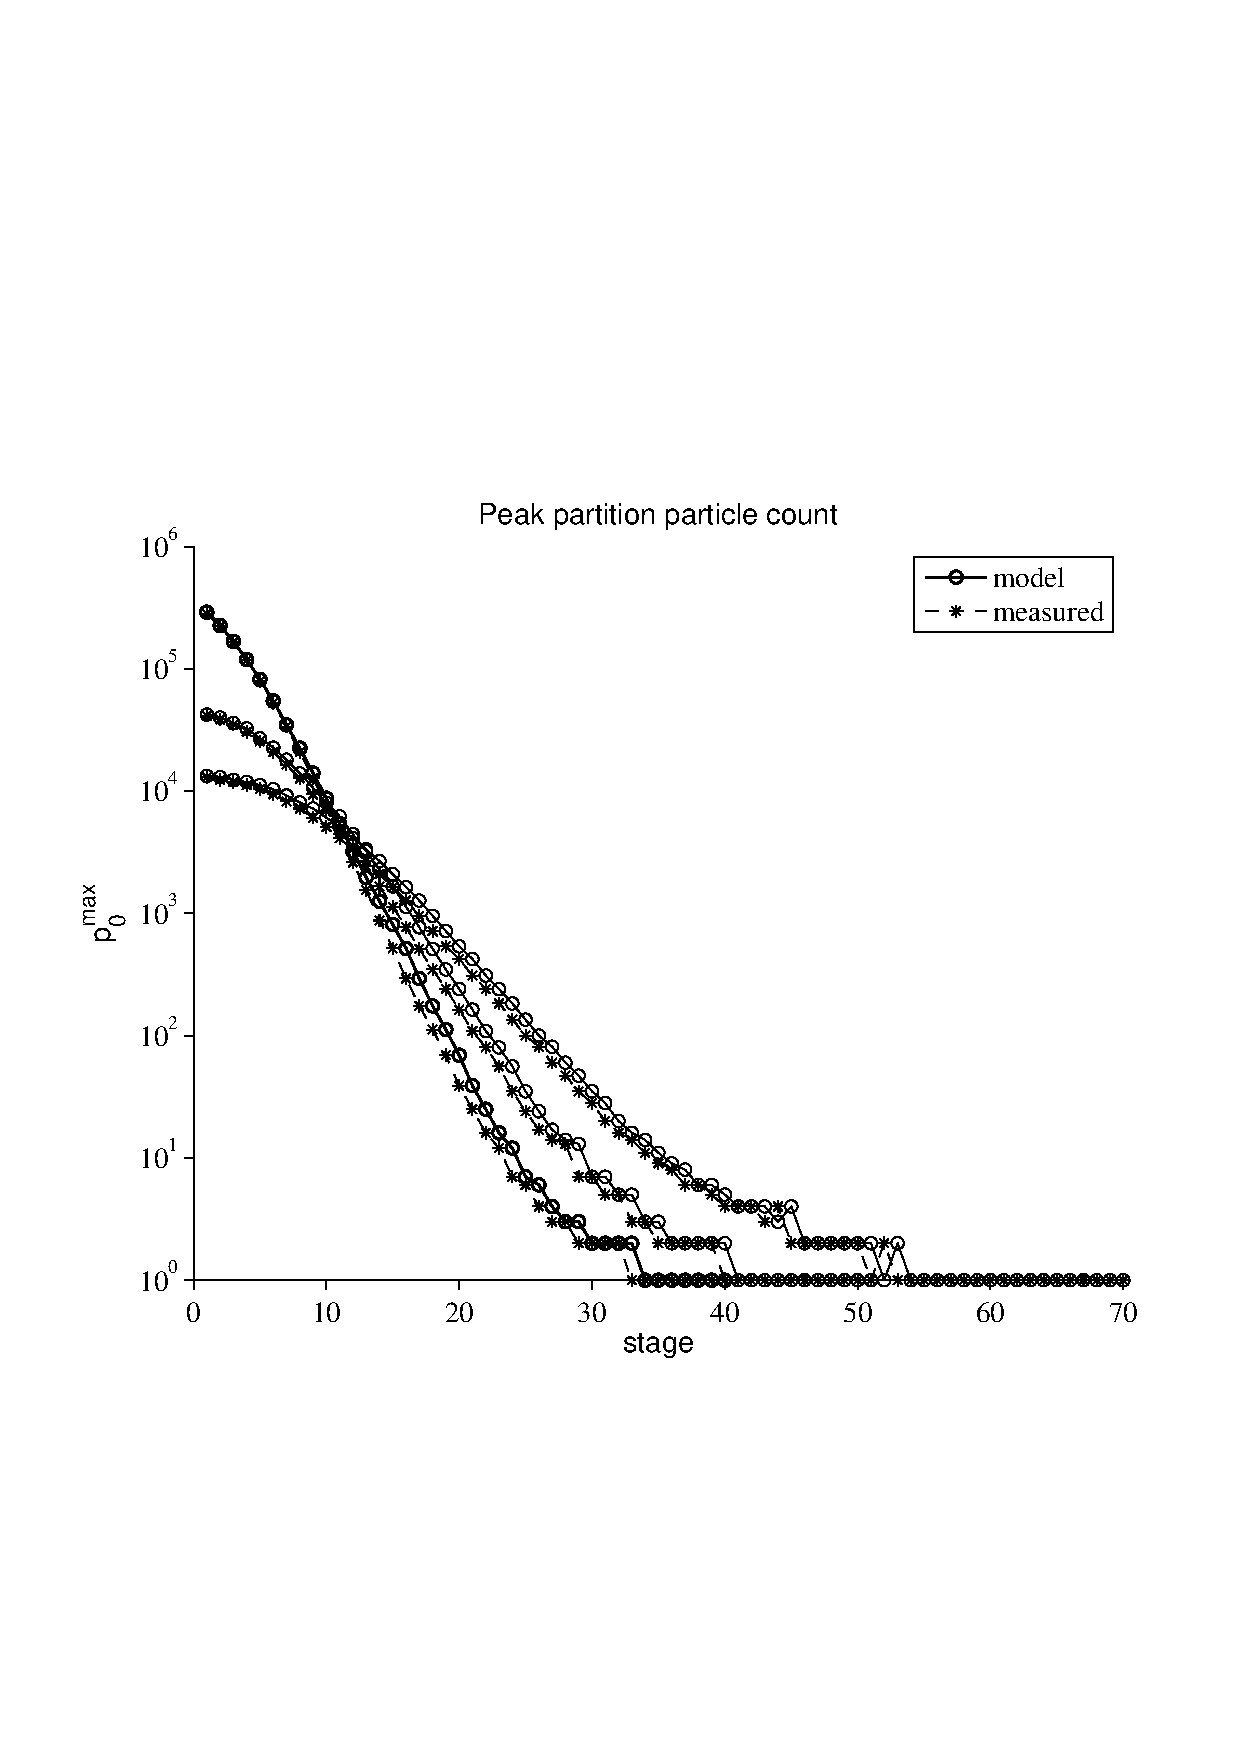
\includegraphics[width=4.0in]{figures/ch5/ub_source.pdf}
  \caption{Average values of leakage rate $\lambda$ at each stage for the full,
    quarter, and ninth assembly experiments. Superposed as error bars are the
    standard deviation, showing very little spatial variation in the early
    stages. The leakage rate trend clearly indicates the higher probability of
    thermalization in later stages of the calculation}
  \label{fig:ub_source}
\end{figure}

\subsection{Evaluation of correction factor $C$ and penalty $\Delta$}
Given an initial particle configuration and reasonable estimates for leakage, it
remains to evaluate $C$ in \eqref{eq:delta5}. To reiterate, under the assumption
of spatially constant leakage $C$ is identically $1$ and the load balance can be
upper bounded by the initial particle configuration as
$\frac{p_0^{max}}{\overline{P_0}}$. When leakage rates vary spatially $C$
measures the amplification of the performance penalty. We estimate $C$ in two
steps, first evaluating the contribution of the bandwidth and tracking times,
given by the ratio
\begin{equation*}
  \frac{\beta ||\lambda^{max}|| + \mu}{\beta ||\overline{\lambda}|| + \mu} =
  \frac{\frac{\beta}{\mu}||\lambda^{max}|| +
    1}{\frac{\beta}{\mu}||\overline{\lambda}|| + 1}.
\end{equation*}
Note that for any conventional machine $\beta << \mu$, reflecting that tracking
rates are much slower than inter-processor communication, and since
$||\overline{\lambda}|| \sim ||\lambda^{max}||$, this term remains very close to
unity and contributes negligibly to the overall load imbalance.

The second contribution of $C$ is the ratio
\begin{equation*}
  \frac{\sum_{i=0}^M ||{\lambda^{max}}||^i}{\sum_{i=0}^M
    ||\overline{\lambda}||^i}.
\end{equation*}
Note that this term becomes problematic as the processor grid is refined, since
we intuitively expect maximum leakage rates of unity for sufficiently small
domains. Assuming that this is the case, the numerator is upper bounded by
$1+M$, where again $M$ is the number of stages in a cycle. Assuming that the
average value does not approach unity, the Taylor series approximation should be
reasonable and we can rewrite this expression as:
\begin{equation*}
  \frac{\sum_{i=0}^M ||{\lambda^{max}}||^i}{\sum_{i=0}^M
    ||\overline{\lambda}||^i} \le M(1-||\overline\lambda||).
\end{equation*}
While this term is likely a modest fraction of the total number of stages, we
must recall that $M$ increases with decreasing partition size, and even a small
fraction could easily significantly amplify the load imbalance.

To explore this in greater depth requires use of the OpenMC simulation
results. \autoref{tab:delta} shows the results, including the model predictions
for the load imbalance penalty for the full, quarter, and ninth assembly
experiments. Note that in all cases the initial particle configuration and thus
$\frac{p_0^{max}}{p_0}$ is expected to be roughly independent of partition size
and be roughly approximated by the one-group solution on a cylindrical
geometry: \[ S(x,y,z) = J_0\left(\frac{2 r_0 x}{L}\right) J_0\left(\frac{2 r_0
  y}{L}\right) \cos\left( \frac{\pi z}{L}\right), \hspace{.2in} \frac{L}{2} \ge
x,y,z \le \frac{L}{2} \] where $r_0=\pm 2.4048$ is the root of the zeroth order
Bessel Function $J_0$. Note that $S$ has a peak to mean value
$\frac{S^{max}}{\overline{S}} = 4.33$, which is reasonably close the values of
$\frac{p_0^{max}}{\overline{P}}$ shown in \autoref{tab:delta}.

\begin{table}
  \centering
  \begin{tabular}{c c c c c c c}
    \toprule
    \emph{experiment} & $\xx$ & $\yy$ & $C$ &
    $\frac{p_0^{max}}{\overline{P_0}}$ & $\Delta$ \\
    \midrule
    full assembly & $1.00$ & $1.13$ & $1.13$ & $3.24$ & $3.67$\\
    quarter assembly & $1.00$ & $2.58$ & $2.58$ & $3.28$ & $8.47$\\
    ninth assembly & $1.00$ & $6.98$ & $6.98$ & $3.45$ & $24.15$\\
    \bottomrule
  \end{tabular}
  \caption{Values of $\Delta$ and the various terms which contribute to it for
    each of the three numerical experiments. The tables used values of inverse
    latency $\beta = 10^{-8} \frac{sec}{particle}$ and tracking time $\mu =
    5\times10^{-4} \frac{sec}{particle}$. Note that within the precision presented
    the bandwidth term (second column) is identical in all cases, a manifestation
    of the fact that bandwidths are much higher than tracking rates. Notice also
    that the load imbalance penalty is magnified significantly on the finest
    partitions grid.}
  \label{tab:delta}
\end{table}

Equation \eqref{eq:delta5} states that, with no load rebalancing, a simulation
with this initial particle distribution is expected to take at most
$C\frac{p_0^{max}}{\overline{P_0}}$ as long as a perfectly load balanced
simulation. For the full assembly simulation $C=1.13$ and the total penalty is
$3.67$, which could in many contexts be considered reasonable compared to
e.g. the cost and complexity of implementing repartitioning algorithms. However,
it is clear that the situation rapidly deteriorates for decreasing partition
size, with a value of $C=6.98$ for the ninth partition experiments. This
corresponds to load imbalance penalty of $24.15$, which for most contexts is
likely unacceptably high. It is clear what has happened both in the model and
the physics --- In the one-ninth assembly case the peak leakage is unity for all
but the final stage, and thus the summation in the numerator of $C$ approaches
$M$. Note that we expect the performance to degenerate even further with
decreasing partition size since M is expected to increase according to
\eqref{eq:kfinal}.

\section{Conclusion}
We have developed simple relationships to quantitatively analyze the impact of
load imbalances on the performance of domain decomposed MC methods in the
context of reactor analysis. These techniques provide a quantitative framework
to estimate the additional performance costs incurred by typical load imbalances
in reactor applications. Preliminary numbers were presented for a classic
reactor benchmark, indicating that load imbalances were not that significant for
assembly-size partitions, but increased dramatically as partition sizes were
decreased beyond that point. This indicates that domain decomposition is likely
a reasonable strategy for modest-size parallelism but that it is inherently
limited when we consider the massive levels of concurrency on the path to
exascale computing (at least without significant repartitioning).

Our main goal however is not to judge here whether these penalties are large or
small in an absolute sense.  Rather, the techniques presented allow one to weigh
tradeoffs between domain decomposition and more sophisticated data decomposition
strategies for their specific needs, or perhaps to estimate the cost of carrying
out load re-balancing or other re-tracking techniques within an operational
production code. When processing power is cheap and memory is at a premium,
factors of several in performance time are not necessarily large, and
performance models that go beyond purely speculative are a critical component of
assessing the best path forward.
